\documentclass[a4paper, 12pt]{article}

\usepackage[T2A]{fontenc}
\usepackage[utf8]{inputenc}
\usepackage[english,russian]{babel}
\usepackage[left=15mm, top=20mm, right=15mm, bottom=20mm, nohead, nofoot]{geometry}

\usepackage{hyperref}
\usepackage{graphicx}
\usepackage{wrapfig}
\usepackage{afterpage}
\usepackage{amsmath, amsfonts, amssymb, amsthm, mathtools}
\author{Хомутов Андрей, группа Б06-903}
\title{ВПВ по курсу "Электричество и магнетизм" \\ Конденсатор на высоких частотах}
\date{22 декабря 2020 г.}
%%%%%%%%%%%%%%%%%%%%%%%%%%%%%%%%%%%%%%%%%%%%%%%%%%%%%%%%%%%%%%%%%%%%%%%%%
\usepackage{graphicx, wrapfig, subcaption, setspace, booktabs}
\usepackage[protrusion=true, expansion=true]{microtype}
\usepackage[english]{babel}
\usepackage{sectsty}
\usepackage{url, lipsum}
\newcommand{\HRule}[1]{\rule{\linewidth}{#1}}
\onehalfspacing
\setcounter{tocdepth}{5}
\setcounter{secnumdepth}{5}
%%%%%%%%%%%%%%%%%%%%%%%%%%%%%%%%%%%%%%%%%%%%%%%%%%%%%%%%%%%%%%%%%%%%%%%%%


\begin{document}

\title{ \normalsize \textsc{Лабораторная работа по физической химии}
		\\ [4.0cm]
		\HRule{0.5pt} \\ [0.3cm]
		\LARGE \textbf{{Электрокапиллярные явления}}
		\HRule{0.5pt} \\ [0.1cm]
		\normalsize  \vspace*{18\baselineskip}}

\date{}

\author{Шамарина Екатерина, Б06-903 \\
		Хомутов Андрей, Б06-903 \\
ФБМФ, 2021\\ }

\maketitle
\thispagestyle{empty}
\newpage
%%%%%%%%%%%%%%%%%%%%%%%%%%%%%%%%%%%%%%%%%%%%%%%%%%%%%%%%%%%%%%%%%%%%%%%%%
\section*{Цели работы} 
\begin{enumerate}
    \item Исследование зависимости поверхностного натяжения на границе ртуть-раствор электролита от электрического потенциала.
    \item Определение потенциала нулевого заряда и емкости двойного электрического слоя на поверхности ртутного электрода в растворе; оценка параметров плотной части д.э.с.
    \item Исследование влияния природы электролита на потенциал нулевого заряда и величину максимального натяжения.
\end{enumerate}
%%%%%%%%%%%%%%%%%%%%%%%%%%%%%%%%%%%%%%%%%%%%%%%%%%%%%%%%%%%%%%%%%%%%%%%%%
\section{Практическая часть}
\subsection{Исследование электрокапиллярной кривой}
Исследование электрокапиллярной кривой на ртути проводилось с помощью измерения краевого угла смачивания декана на поверхности ртути в водном растворе 0.1M NaF по трёхэлектродной схеме. \newline
После нанесения капли декана(5мкл) на пов-ть ртути была проведена тренировка капли. (Потенциал ртутного электрода от 300 до –1300 мВ относительно хлорсеребряного электрода в циклическом режиме со скоростью развертки 50 мВ/с.) \newline
Произведены измерения краевого угла смачивания от величины потенциала ртутного электрода.(Рез-ты в Табл.1.) Далее из уравнения Юнга получены значения поверхностного натяжения на границе вода-ртуть. 
$$\sigma_{\text{вр}} = \sigma_{\text{др}} + \sigma_{\text{дв}} cos\theta$$

\begin{table}[h!]
\begin{center}
\caption{Результаты измерений}
\begin{tabular}{|r|l|l|l}
\cline{1-3}
\multicolumn{1}{|l|}{E, mV} & \theta,deg    & \sigma, mN/m  &  \\ \cline{1-3}
-1300                       & 106.2 & 360.7715 &  \\ \cline{1-3}
-1201                       & 95.2  & 370.3777 &  \\ \cline{1-3}
-1102                       & 77.1  & 386.3858 &  \\ \cline{1-3}
-1002                       & 60.8  & 399.8808 &  \\ \cline{1-3}
-900.6                      & 50.2  & 407.6456 &  \\ \cline{1-3}
-802                        & 33.8  & 417.3802 &  \\ \cline{1-3}
-702                        & 29.6  & 419.3442 &  \\ \cline{1-3}
-601                        & 25.5  & 421.0318 &  \\ \cline{1-3}
-503                        & 24.8  & 421.2967 &  \\ \cline{1-3}
-404                        & 22.4  & 422.1518 &  \\ \cline{1-3}
-302                        & 24.4  & 421.4449 &  \\ \cline{1-3}
-202                        & 29.7  & 419.3002 &  \\ \cline{1-3}
-102                        & 39.2  & 414.5222 &  \\ \cline{1-3}
0                           & 49.6  & 408.0541 &  \\ \cline{1-3}
102                         & 62.0  & 398.9430 &  \\ \cline{1-3}
199                         & 78.6  & 385.0805 &  \\ \cline{1-3}
298                         & 84.6  & 379.7995 &  \\ \cline{1-3}
399                         & 88.4  & 376.4240 &  \\ \cline{1-3}
\end{tabular}
\end{center}
\end{table}

По полученным данным построен график зависимости $\sigma$(E).
\begin{figure}[h!]
    \begin{center}
    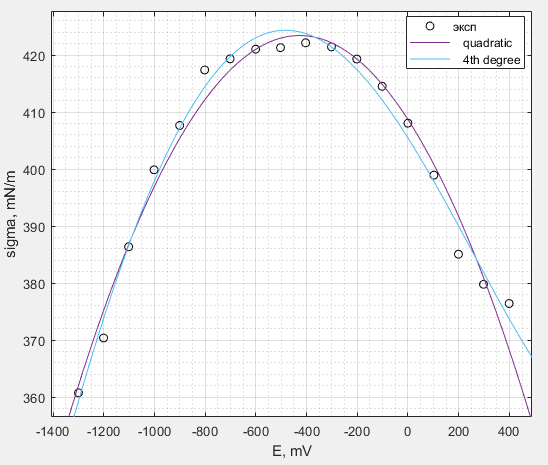
\includegraphics[width=0.8\textwidth]{1 sigma(U)+poly.png}
    \end{center}
    \caption{Электрокапиллярная кривая}
\end{figure}
ПНЗ может быть определён напрямую из графика(тчк максимума) :$\varphi_0 \simeq -400mV$. Также м.б.определён из аппроксимации кривой второй или четвёртой степенью:\newline
$\sigma_2 = -8.06\cdot10^{-5}E^2 - 0.069E + 409 \Rightarrow \varphi_{02} = -428mV$\newline
$\sigma_4 = 1.64\cdot10^{-11}E^4 + 4.96\cdot10^{-8}E^3 - 4.47\cdot10^{-5}E^2 - 0.0705E + 405 \Rightarrow \varphi_{04} = -483mV$

Если представить двойной слой в виде плоского конденсатора, то его удельную ёмкость в ПНЗ можно найти по формуле: $C_s = -\frac{d^2\sigma}{dE^2} \bigg| _{q=0}$ \newline
$C_2 \simeq 16 \frac{\text{мкФ}}{\text{см}^2}$     
$C_4 \simeq 18 \frac{\text{мкФ}}{\text{см}^2}$

По полученной ёмкости можно оценить расстояние между обкладками конденсатора: $d = \frac{\epsilon \epsilon_0}{C_s} = \frac{4 \cdot 8.85\cdot 10^{-12} \frac{\text{Ф}}{\text{м}}}{0.17\frac{\text{Ф}}{\text{м}^2}} \simeq 2.1 \buildrel _\circ \over {\mathrm{A}}$

Соотнесём оценку с теориями Гельмгольца и Гуи-Чапмена строения двойного электрического слоя.

Гельмгольц) $C_{\text{пл}} = \frac{\epsilon \epsilon_0}{r}$, где r - радиус гидратированного иона, может быть найден из модели Стокса: $r = \frac{1}{6\pi\eta b} = \frac{eF}{6\pi\eta\lambda^0}$ = 1.63$\buildrel _\circ \over {\mathrm{A}}$ для $Na^+$ и 1.48$\buildrel _\circ \over {\mathrm{A}}$ для $F^-$\footnote{$\lambda_{Na}=50.28\cdot10^{-4}$ и $\lambda_F=55.4\cdot10^{-4} \frac{m^2}{\Omega mol}$соотв, Сухотин А.М. Справочник по электрохимии} Оба этих значения меньше оценочных 2.1 $\buildrel _\circ \over {\mathrm{A}}$. ДЭС удовлетворял бы приближению Гельмгольца, если бы $\epsilon \simeq 2.9$.

Гуи-Чапмен) $C_d = \sqrt{C_\infty} \sqrt{\frac{2\epsilon \epsilon_0 F^2}{RT}} ch\left( \frac{zF\varphi}{2RT} \right) \simeq \sqrt{C_\infty} \sqrt{\frac{2\epsilon \epsilon_0 F^2}{RT}} \simeq 73 \frac{\text{мкФ}}{\text{см}^2}$

Тогда воспользуемся моделью Штерна: $C_\text{пл} = \frac{C \cdot C_d}{C_d - C} \simeq 22 \frac{\text{мкФ}}{\text{см}^2}$. В этом случае $d \simeq 1.59 \buildrel _\circ \over {\mathrm{A}}$ что хорошо согласуется с радиусами гидратированных ионов и, соответственно, толщиной ДЭС в модели Гельмгольца.














\subsection{Исследование поляризуемости Hg-электрода}
Измерения проводились при концентрации NaF = 0.1 M. Сначала была снята ЦВАХ рабочего электрода в диапазоне от -2.3 до 0.3 В. Потенциал разрыва цепи составил около 70 мВ, с течением времени он дрейфовал.
\begin{figure}[h!]
    \begin{center}
    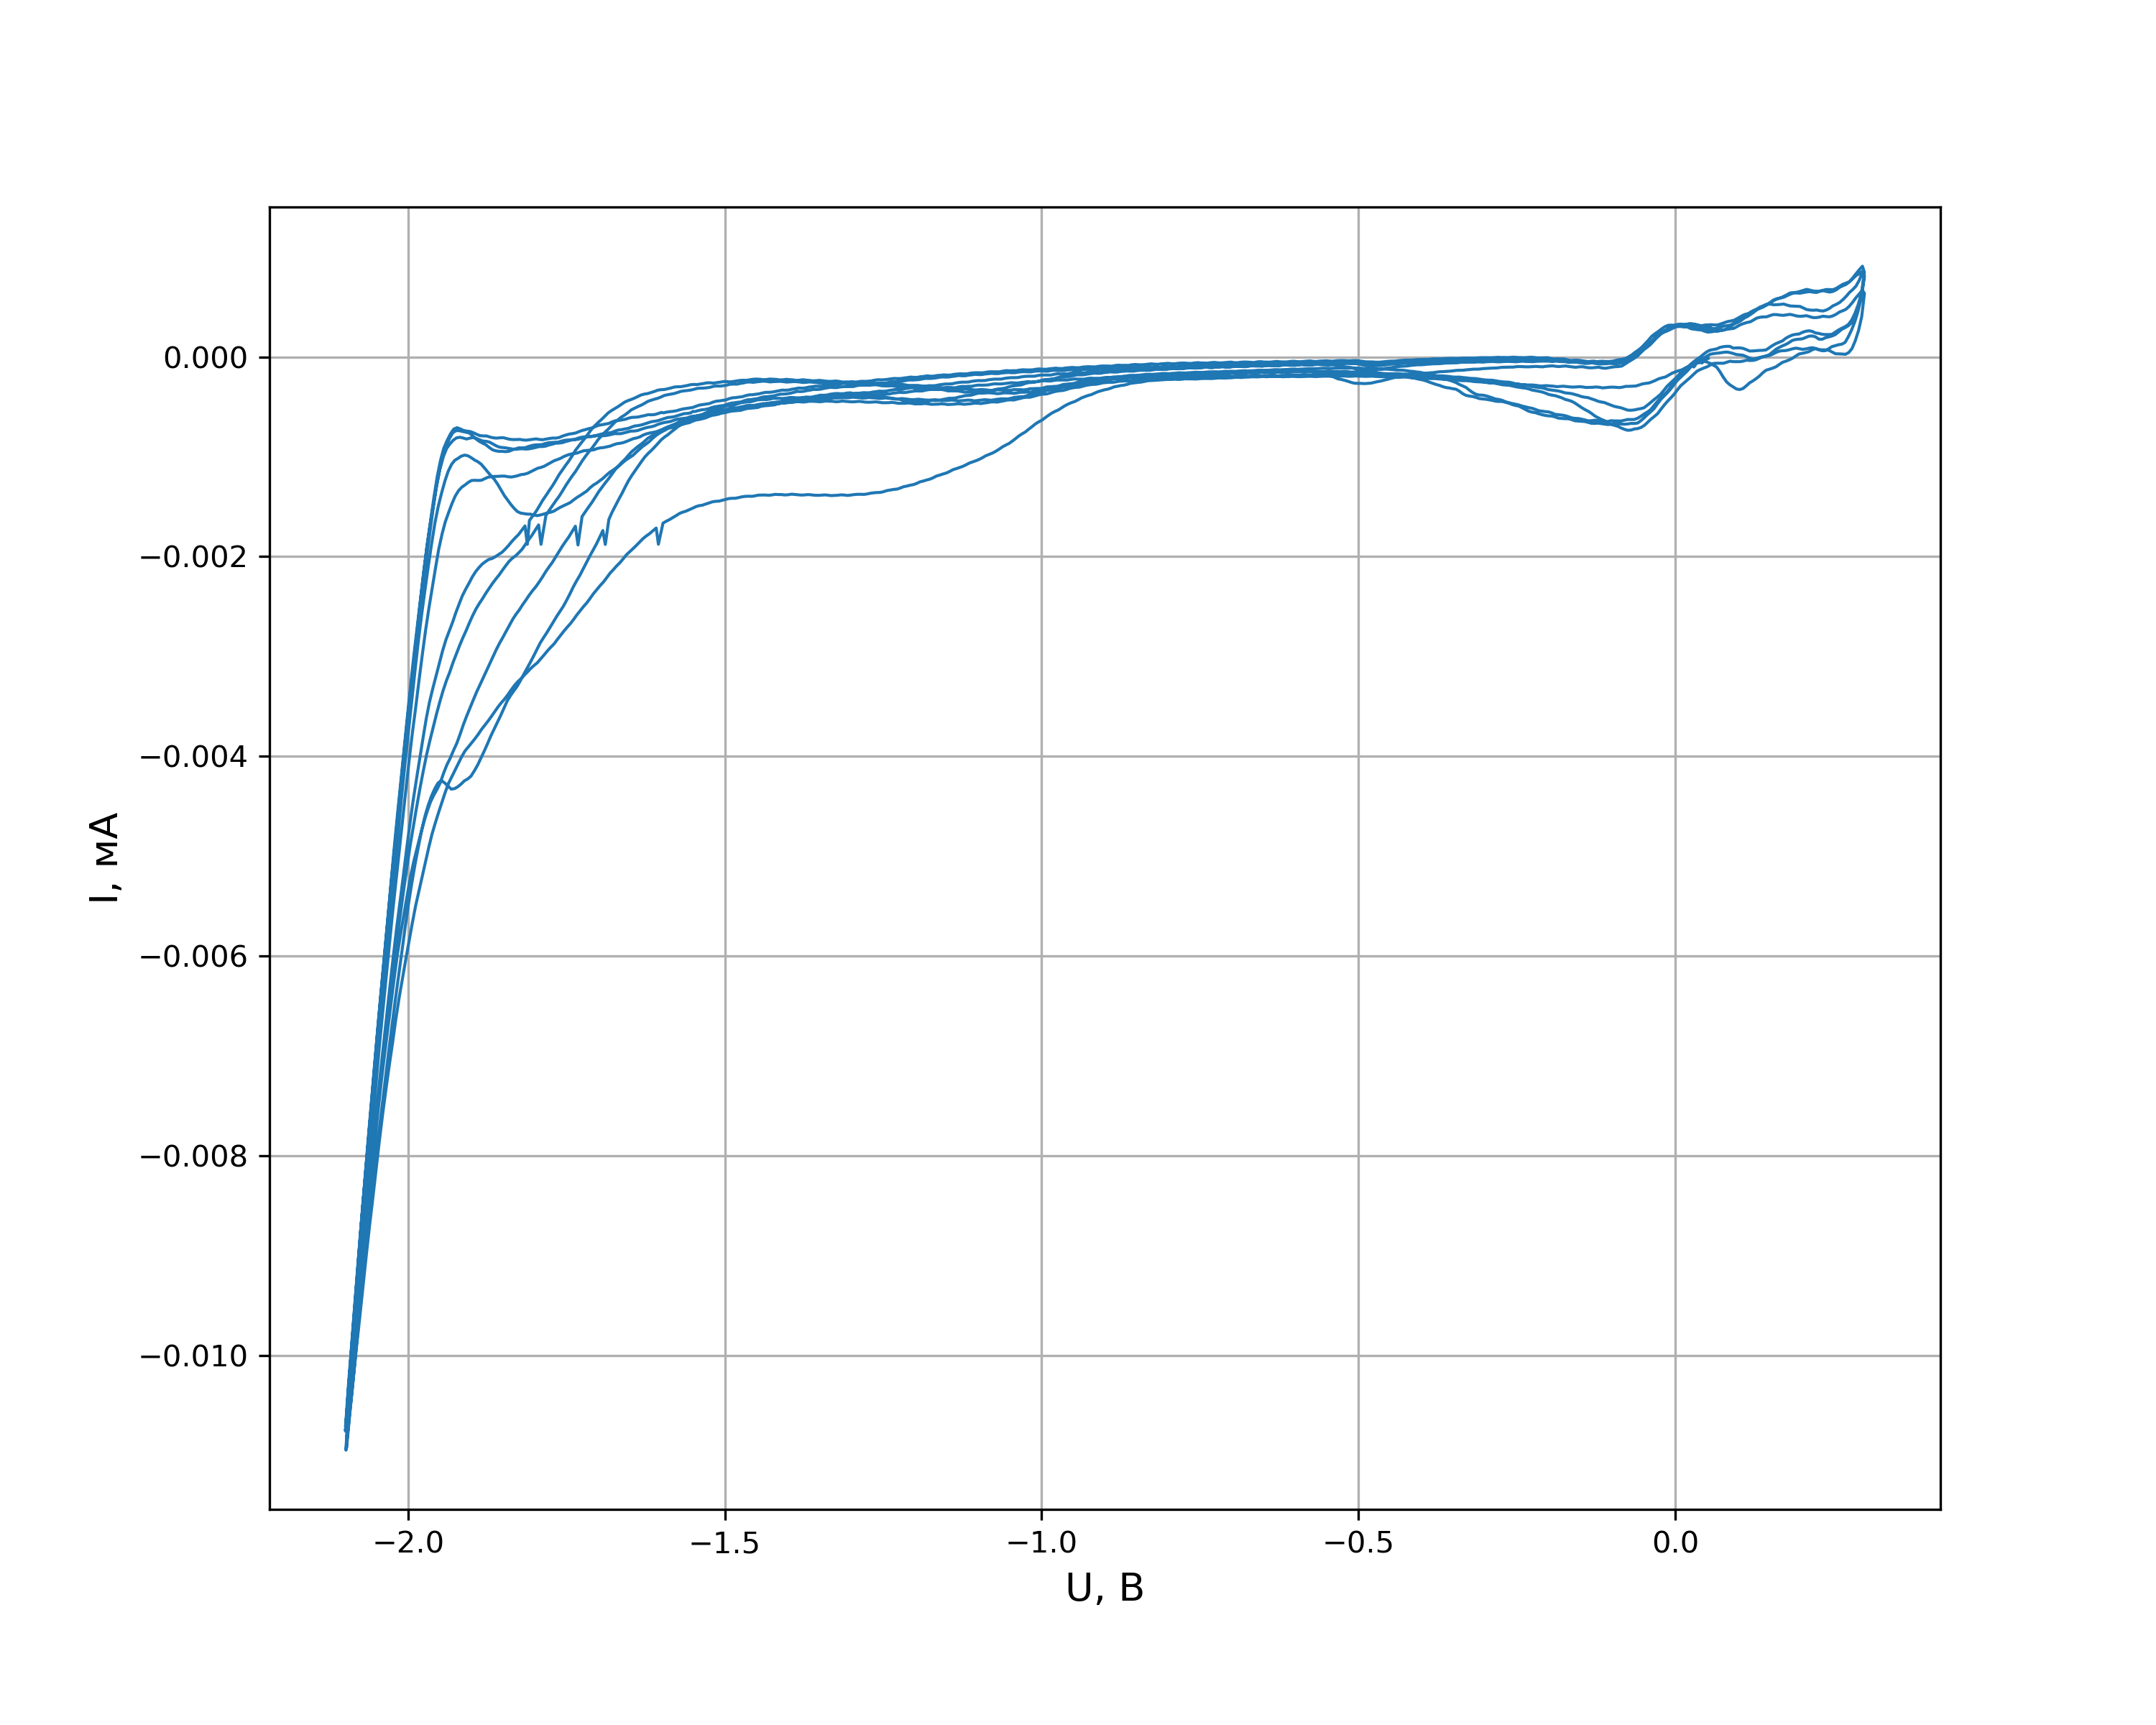
\includegraphics[width=0.8\textwidth]{A.png}
    \end{center}
    \caption{ЦВАХ ртутного эл-да}
\end{figure}

Затем ртутный электрод был выдержан при потенциале -2.3 В относительно вспомогательного хлорсеребряного в течении 3 минут. При этом происходит восстановление натрия с переходом его в ртуть. Потенциал разрыва цепи установился на значении -2027 мВ

Было проведено измерение ЦВАХ ртути в диапазоне потенциалов от -2.3 до -1.8 В и от -2.1 до 0.3 В относительно хлорсеребряного электрода сравнения.

Видно, что получившаяся "батарейка" разряжается до определенного момента, пока весь натрий не перейдет из амальгамы в окисленную форму (при этом можно наблюдать бурное выделение водорода), затем ЦВАХ возвращается к первоначальному и снова можно наблюдать область поляризуемости.

\begin{figure}[h!] %% ШАБЛОН ДЛЯ ДВУХ КАРТИНОК
\begin{center}
\begin{minipage}[h]{0.49\linewidth}
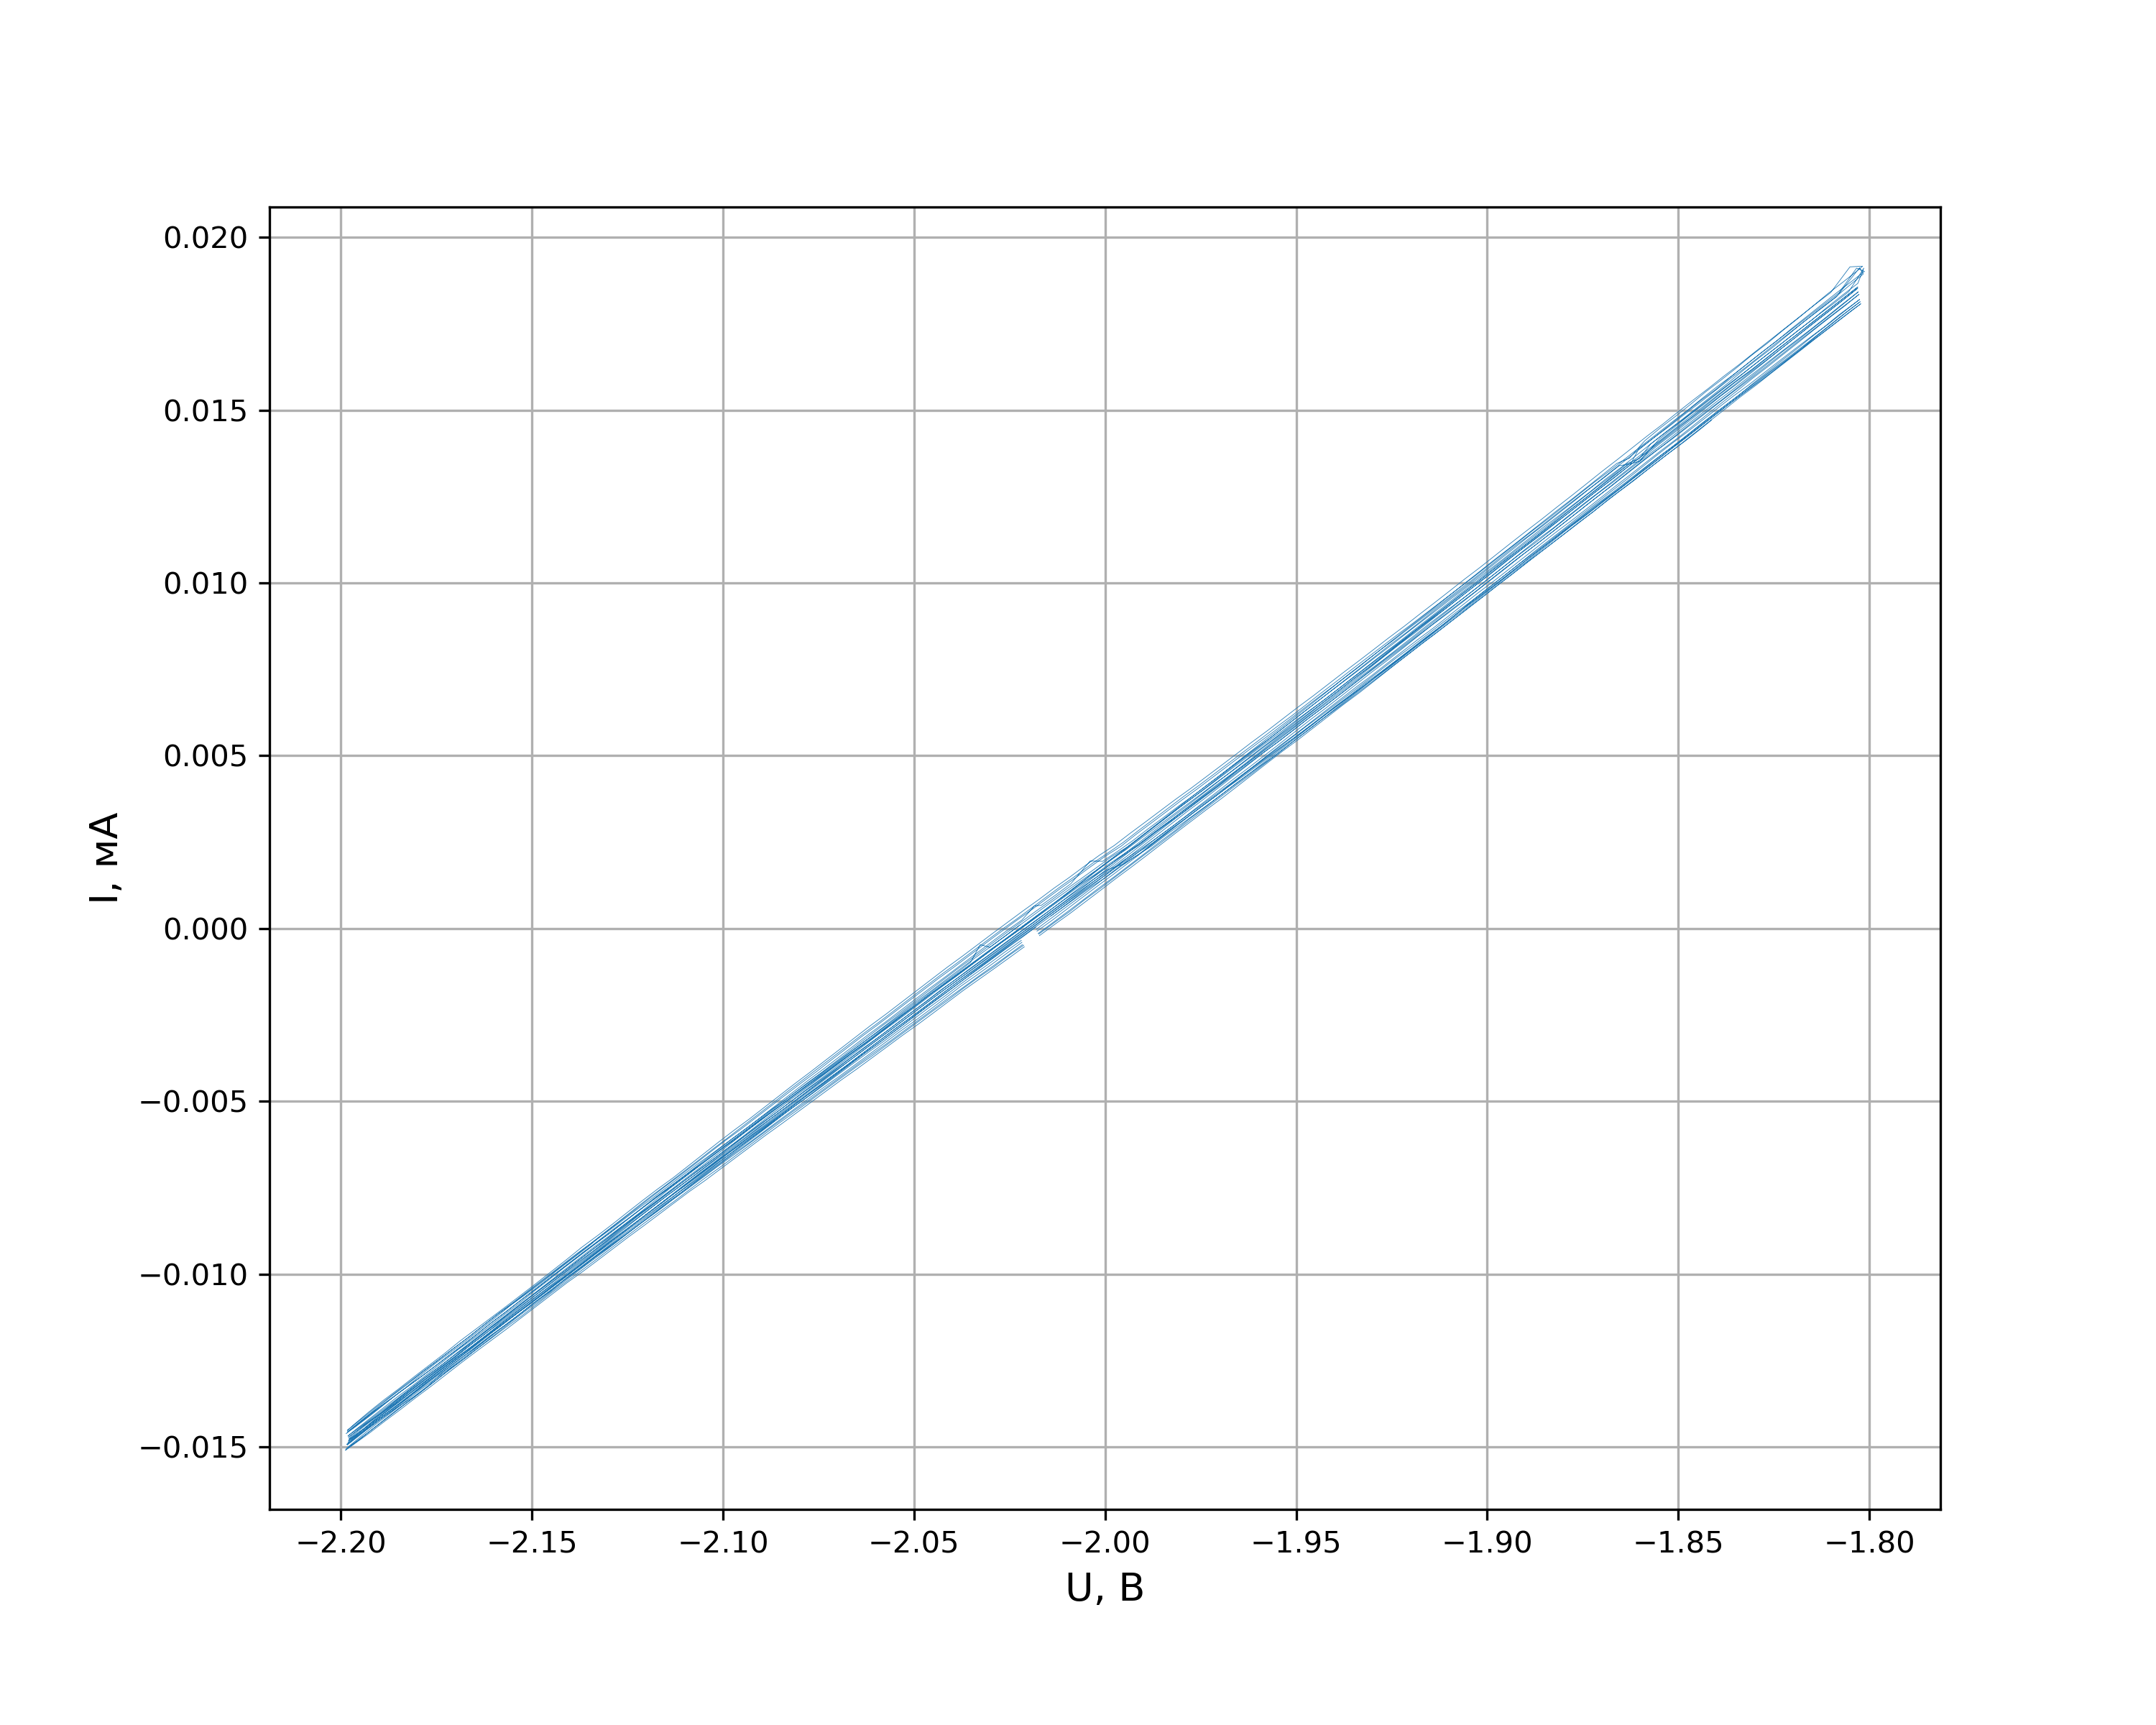
\includegraphics[width=1\linewidth]{C.png}
\caption{ЦВАХ обработанного Hg эл-да (I)} %% подпись к рисунку
\label{ris:experimoriginal} %% метка рисунка для ссылки на него
\end{minipage}
\hfill 
\begin{minipage}[h]{0.49\linewidth}
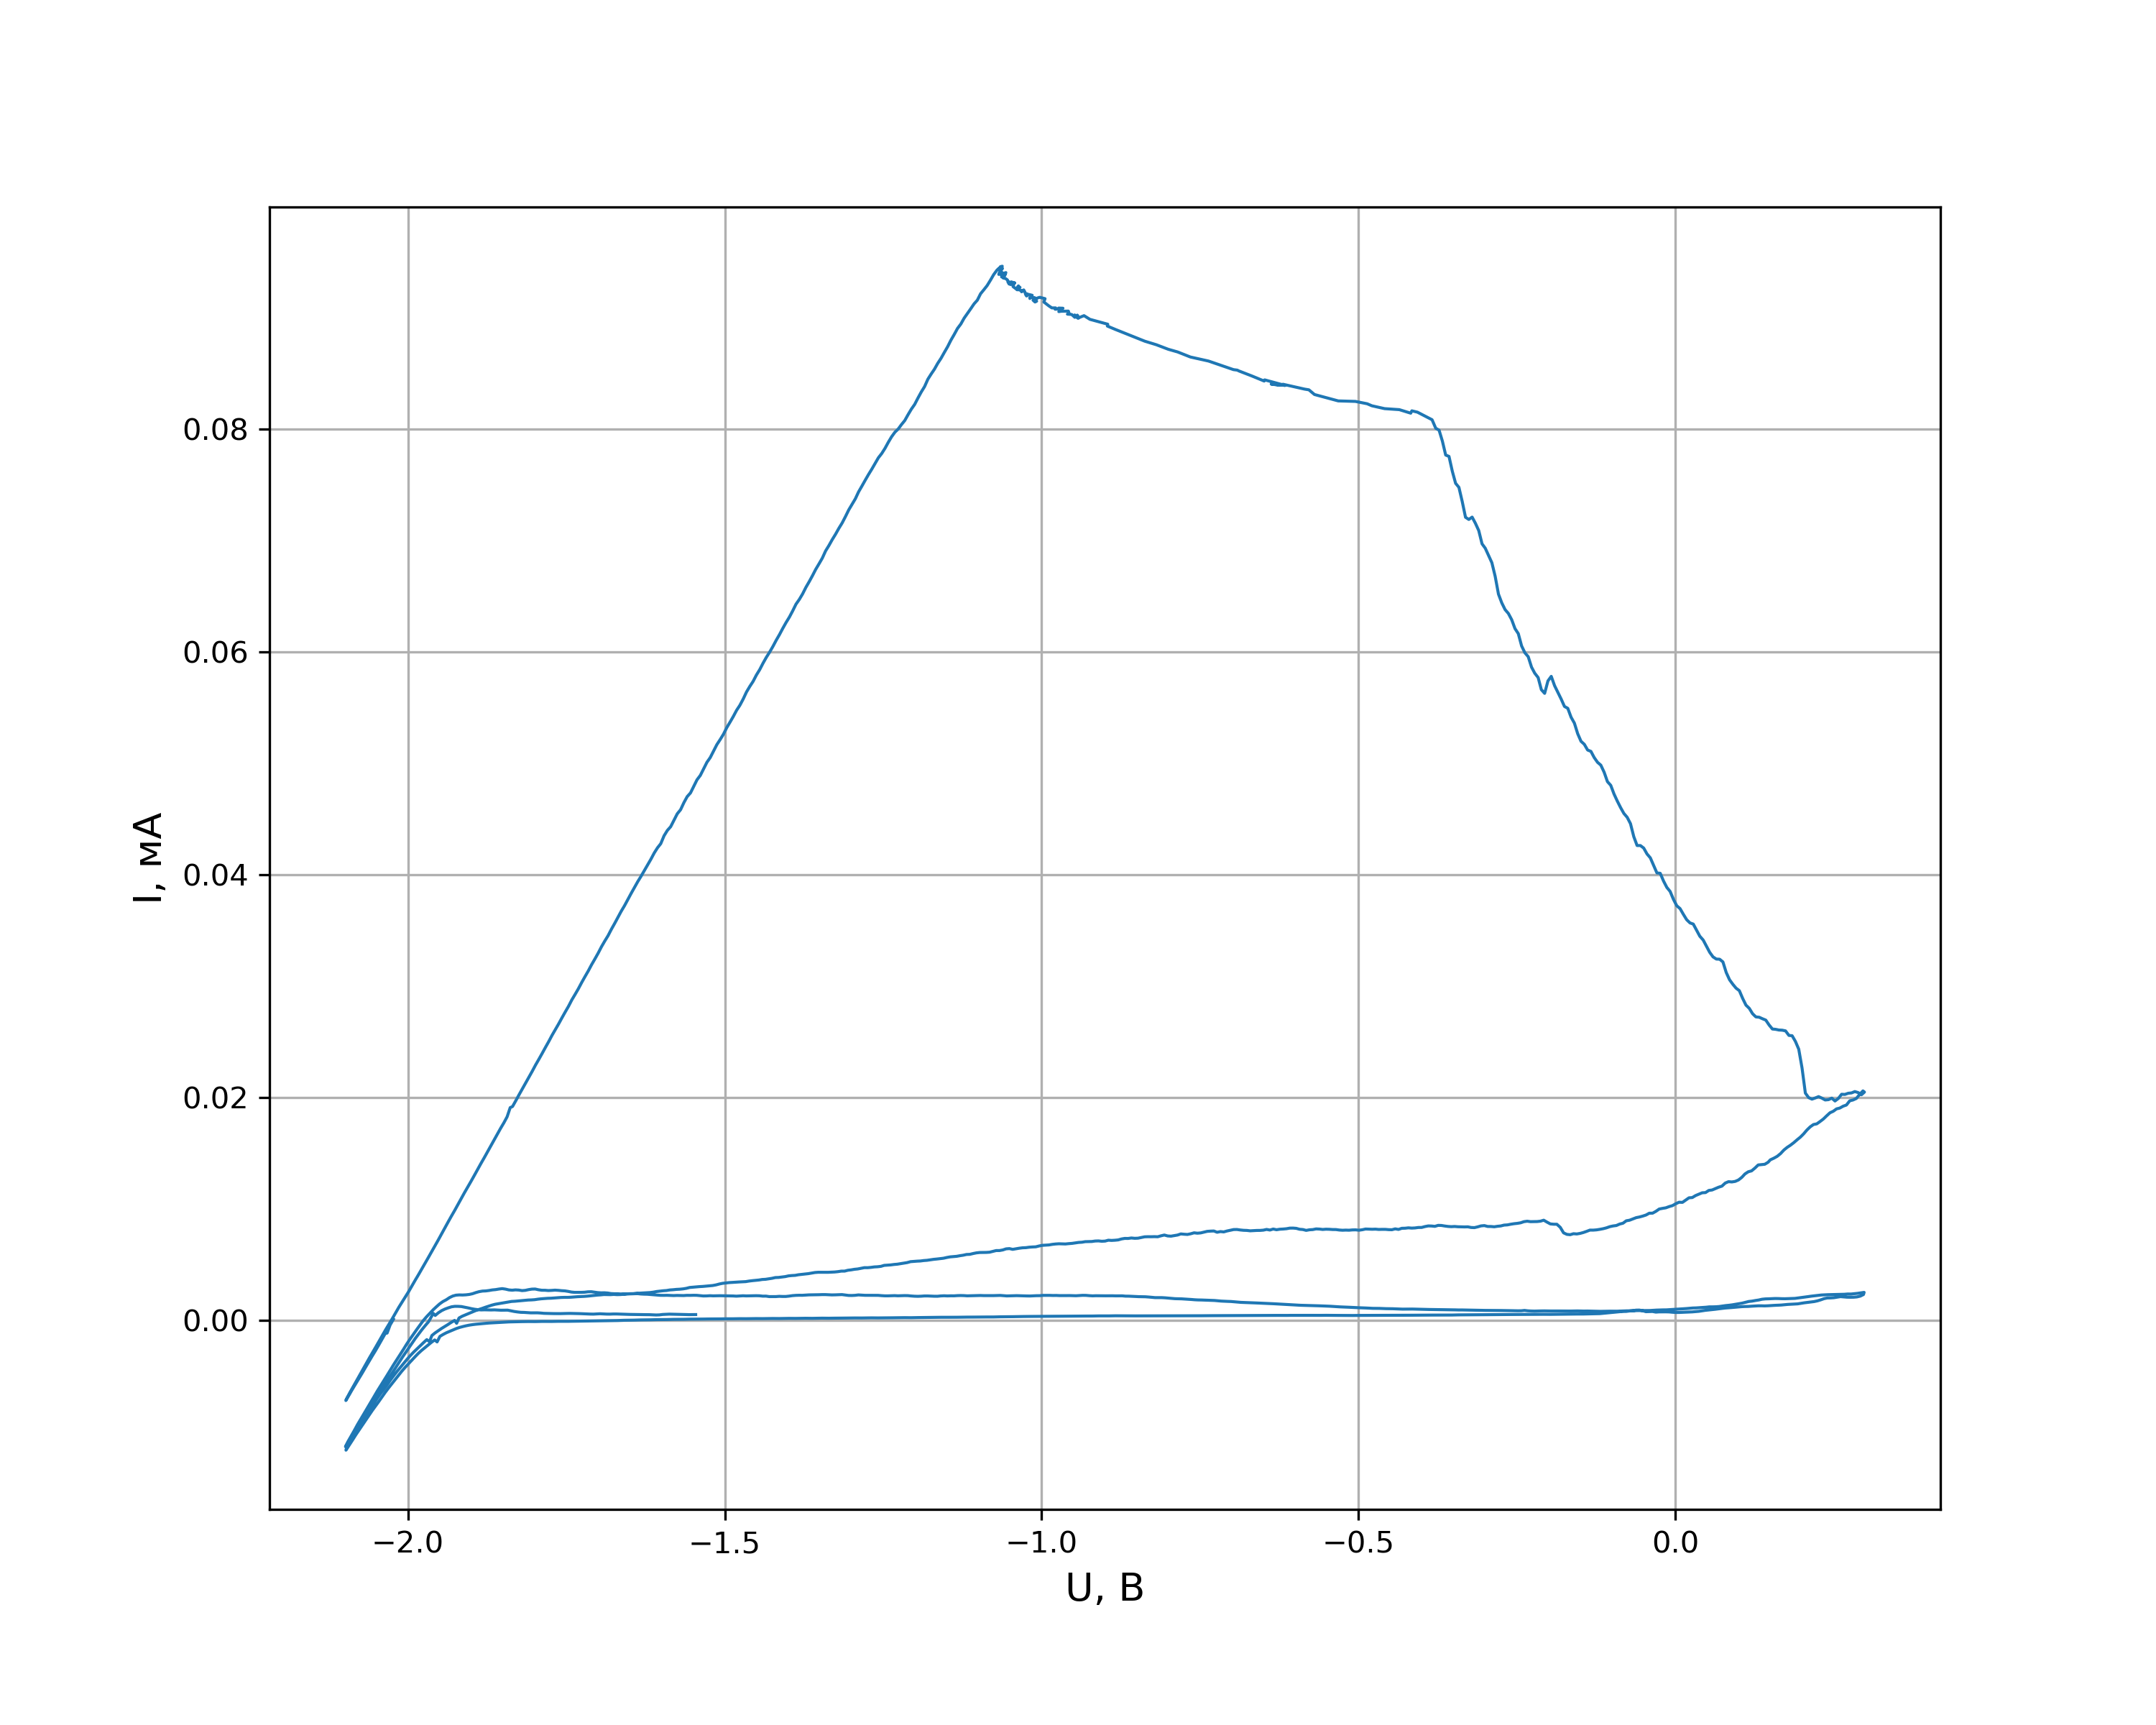
\includegraphics[width=1\linewidth]{D.png}
\caption{ЦВАХ обработанного Hg эл-да (II)}
\label{ris:experimcoded}
\end{minipage}
\end{center}
\end{figure}



%%%%%%%%%%%%%%%%%%%%%%%%%%%%%%%%%%%%%%%%%%%%%%%%%%%%%%%%%%%%%%%%%%%%%%%%%
 \section{Выводы}
\begin{enumerate}
    \item С помощью электрокапиллярной кривой измерен пнз ртути в растворе 0.1M NaF: -428мВ (по аппроксимации полиномом 2 степени) (отн. нас. ХС электрода). Справочное значение: -428мВ.
    \item Оценена ёмкость ДЭС. Оценка удовлетворяет модели Штерна.
    \item Была изменена поляризуемость (на обратимость) ртутного электрода, путем растворения в нем натрия, затем поляризуемость была восстановлена, после переведения натрия обратно в раствор

\end{enumerate}

\end{document}



\begin{table}[h!]
\begin{center}
\caption{...}
\begin{tabular}{|c|c|c|c|c|}

\end{tabular}
\end{center}
\end{table}


\begin{figure}[h!]
    \begin{center}
    \includegraphics[width=0.8\textwidth]{xxx.png}
    \end{center}
    \caption{...}
\end{figure}

\begin{figure}[h!] %% ШАБЛОН ДЛЯ ДВУХ КАРТИНОК
\begin{center}
\begin{minipage}[h]{0.40\linewidth}
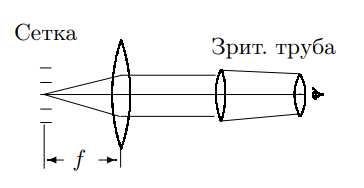
\includegraphics[width=1\linewidth]{plus_lens.PNG}
\caption{...} %% подпись к рисунку
\label{ris:experimoriginal} %% метка рисунка для ссылки на него
\end{minipage}
\hfill 
\begin{minipage}[h]{0.40\linewidth}
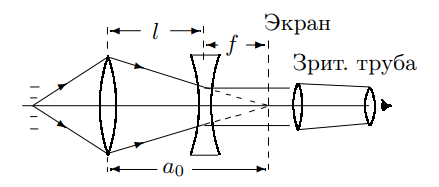
\includegraphics[width=1\linewidth]{minus_lens.PNG}
\caption{..}
\label{ris:experimcoded}
\end{minipage}
\end{center}
\end{figure}







